%% 4 Lorenzo
%4. Shopping Cart page. Where the user can:
%    a. Review all the products he selected;
%    b. Review the the total price and total sales tax;
%    c. Proceed to the checkout;
\subsection{UC10 - Visualizzazione prodotti nel carrello}
\label{UC10}

\begin{figure}[H]
    \centering
    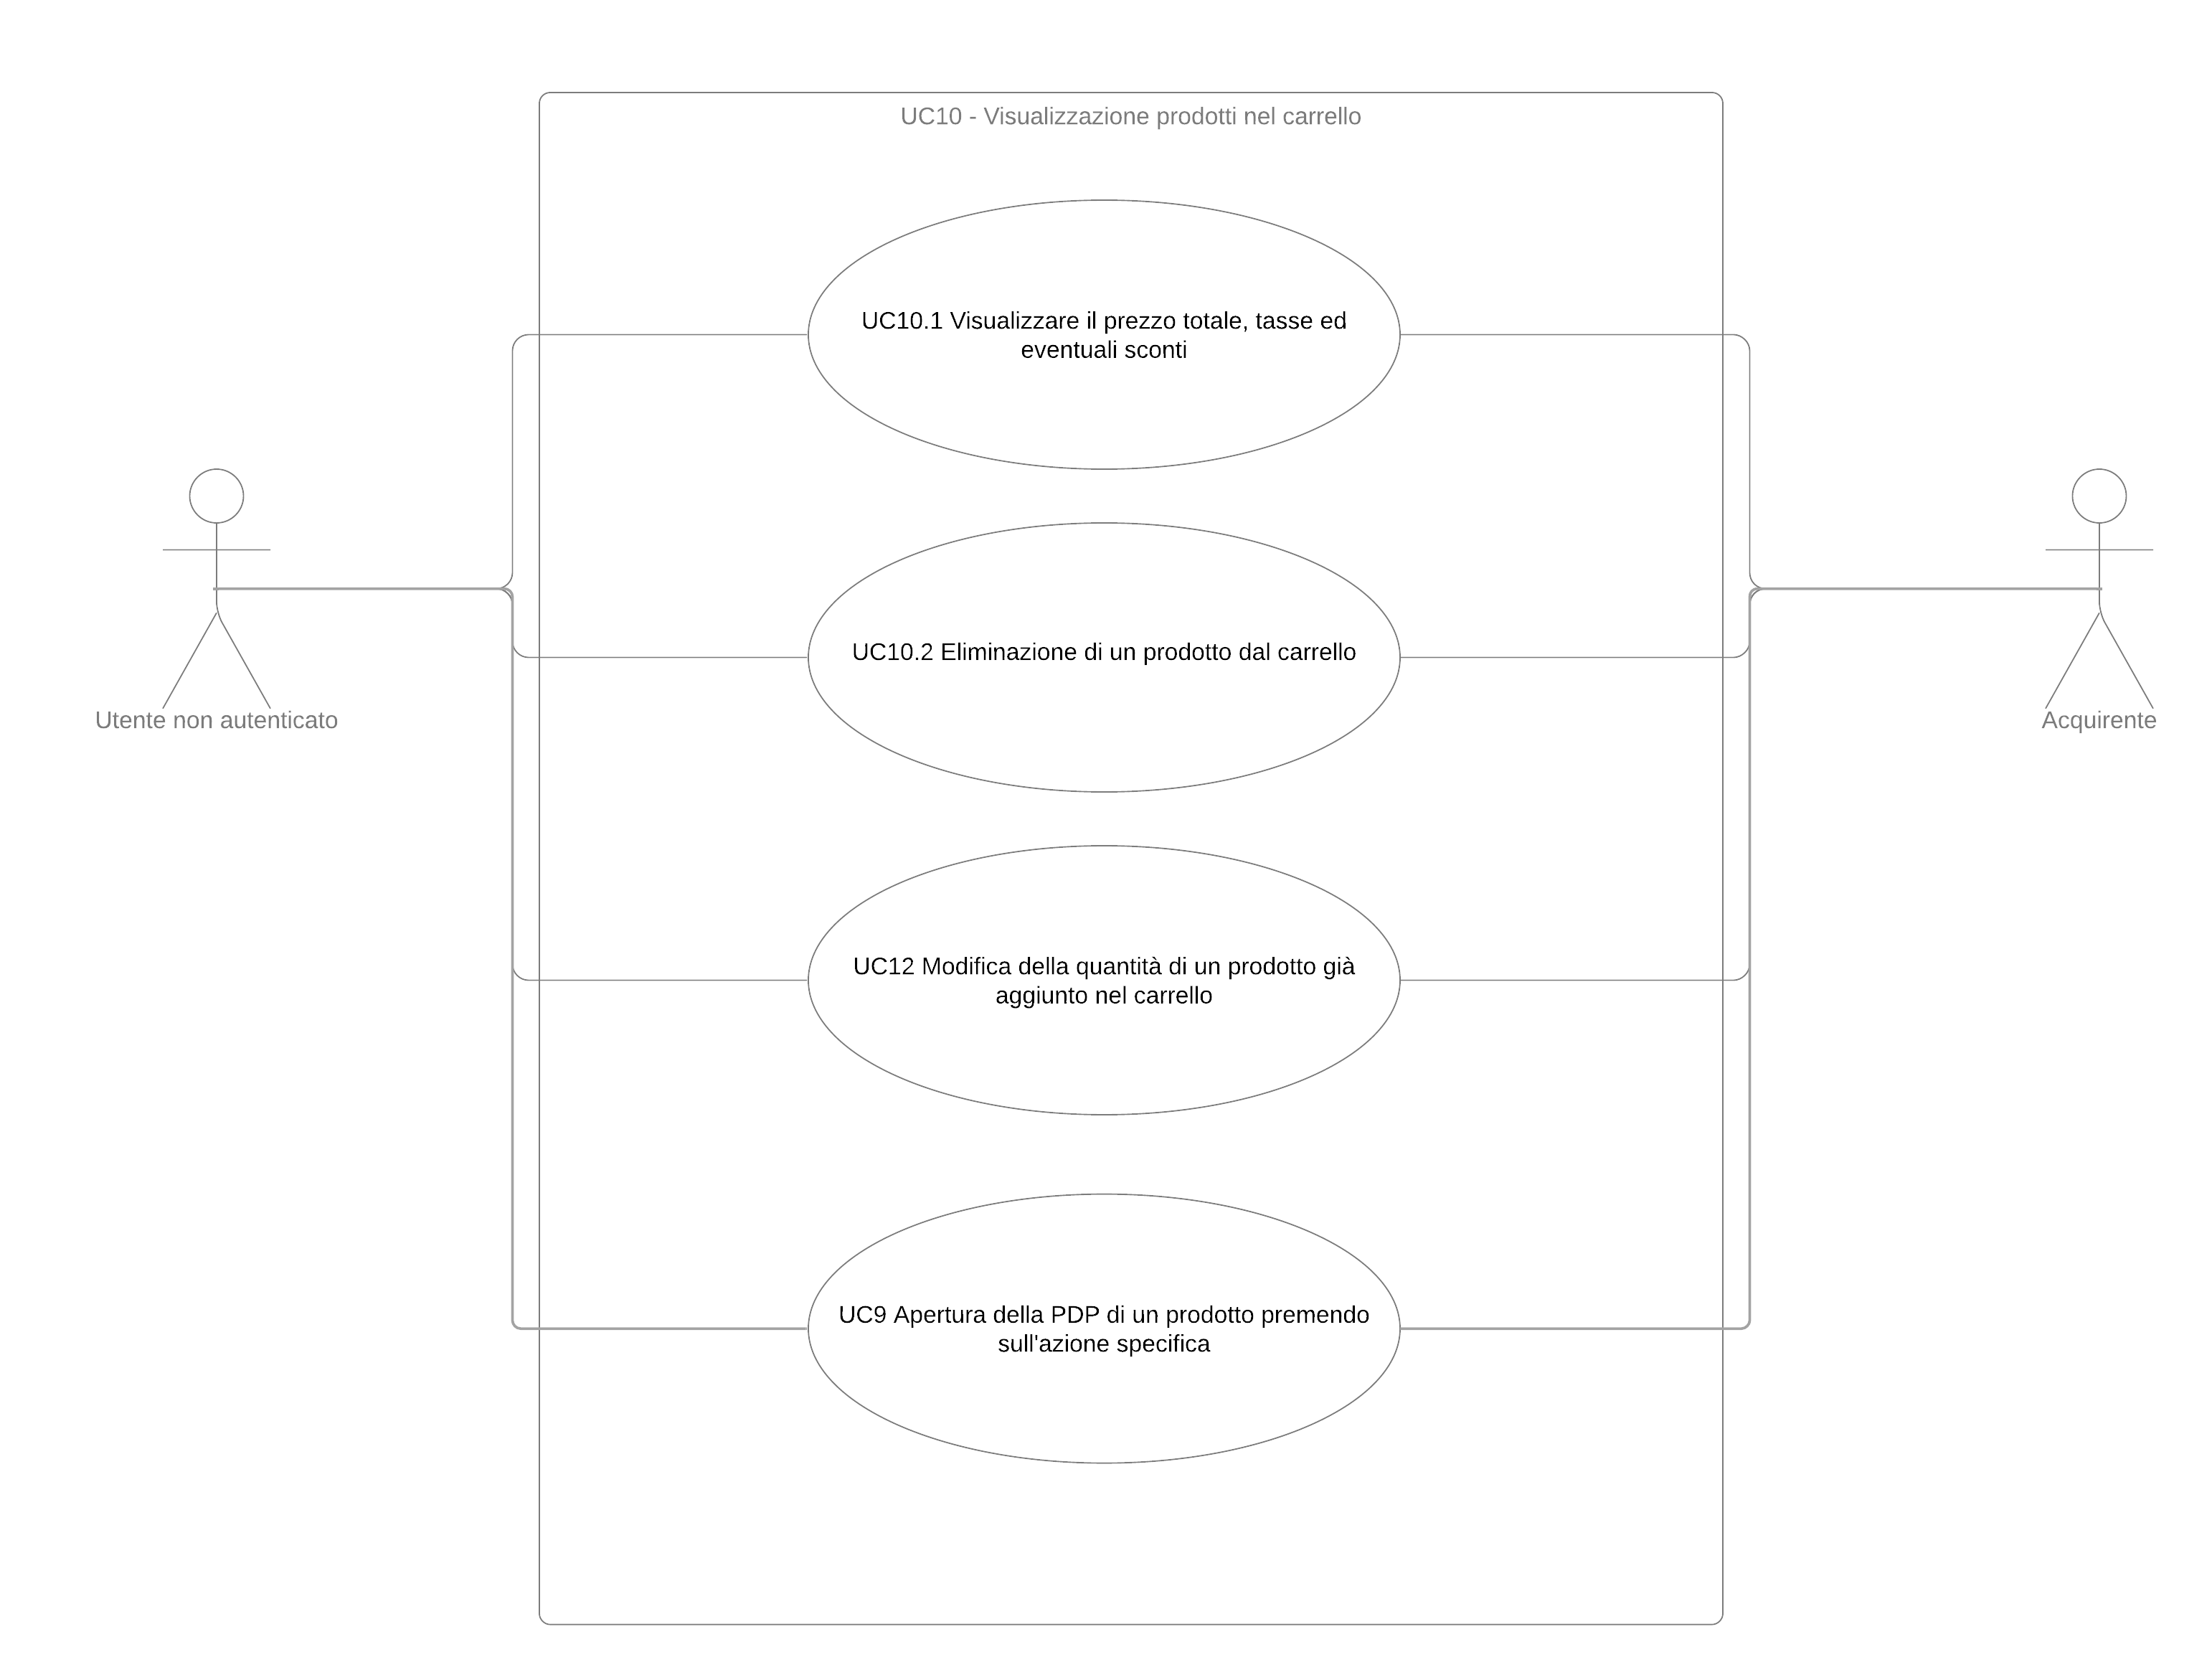
\includegraphics[width=\textwidth]{Immagini/DiagrammiUC/UC10VisualizzazioneProdottiNelCarrello.png}
    \caption{Diagramma di UC10: Visualizzazione prodotti nel carrello} 
    \label{fig:VisualizzazioneProdottiNelCarrello}
\end{figure}
\newpage
L'utente vuole visualizzare i prodotti che ha inserito nel carrello.
\begin{itemize}
    \item \textbf{Attori Primari:} Acquirente; Utente non autenticato.
    \item \textbf{Precondizione:} L'attore si trova nella pagina del carrello.
    \item \textbf{Postcondizione:} L'attore visualizza l'elenco di prodotti che ha messo nel carrello.
    \item \textbf{Scenario Principale:} L'utente clicca sull'azione per entrare nella pagina del carrello all'interno del menù (UC3.4) e vede la lista dei prodotti che sono stati inseriti. Da qui potrà svolgere le seguenti operazioni:
    \begin{itemize}
        \item (UC10.1) - Visualizzare il prezzo totale, tasse ed eventuali sconti.
        \item (UC10.2) - Eliminazione di un prodotto dal carrello.
        \item (UC12) - Modifica della quantità di un prodotto già aggiunto nel carrello.
        \item (UC9) - Apertura della PDP di un prodotto premendo sull'azione specifica.
    \end{itemize}
    \item \textbf{Scenario Alternativo:} Non ci sono prodotti all'interno del carrello, verrà visualizzato il messaggio "Carrello vuoto" e sarà data la possibilità all'attore di andare alla home per iniziare gli acquisti.
\end{itemize}

\subsubsection{UC10.1 - Visualizzazione prezzo totale, tasse ed eventuali sconti} \label{UC10.1}
L'utente vuole vedere l'ammontare delle tasse, la presenza di sconti e il prezzo totale della merce nel carrello.
\begin{itemize}
    \item \textbf{Attori Primari:} Utente non autenticato; Utente autenticato.
    \item \textbf{Precondizione:} L'attore si trova nella pagina del carrello con almeno un prodotto al suo interno.
    \item \textbf{Postcondizione:} Viene calcolato l'ammontare delle tasse, la quantità di sconto e il costo totale e vengono visualizzati dall'utente.
    \item \textbf{Scenario Principale:} Appena l'utente entra nella pagina del carrello, se vi sono presenti dei prodotti, il sistema calcola l'ammontare delle tasse, la quantità di sconto da applicare (in caso sia stato applicato uno sconto) e il prezzo totale dell'ordine.
    \item \textbf{Scenario Alternativo:} Non ci sono prodotti all'interno del carrello non verrà calcolato nessun importo e, di conseguenza, non potrà essere visto dall'utente.
\end{itemize}

\subsubsection{UC10.2 - Eliminazione di un prodotto dal carrello}
\label{UC10.2}
L'acquirente o l'utente non autenticato può eliminare un prodotto che ha inserito nel carrello.
\begin{itemize}
    \item \textbf{Attori Primari:} Acquirente; Utente non autenticato.
    \item \textbf{Precondizione:} L'attore è nella pagina del carrello e ha inserito almeno un prodotto.
    \item \textbf{Postcondizione:} L'attore ha rimosso totalmente il prodotto dal carrello, perciò anche se era selezionato in maggiore quantità.
    \item \textbf{Scenario Principale:} L'attore non vuole più ordinare un prodotto che ha aggiunto nel carrello e, per farlo, svolge le seguenti operazioni:
    \begin{itemize}
        \item Clicca sull'azione di eliminazione del prodotto dal carrello.
        \item Il prodotto viene rimosso dal carrello.
    \end{itemize}
\end{itemize}

%% AGGIUNTA DI FILIPPO E LEONARDO v
\subsection{UC11 - Aggiunta del prodotto al carrello}
\label{UC11}

\begin{figure}[H]
    \centering
    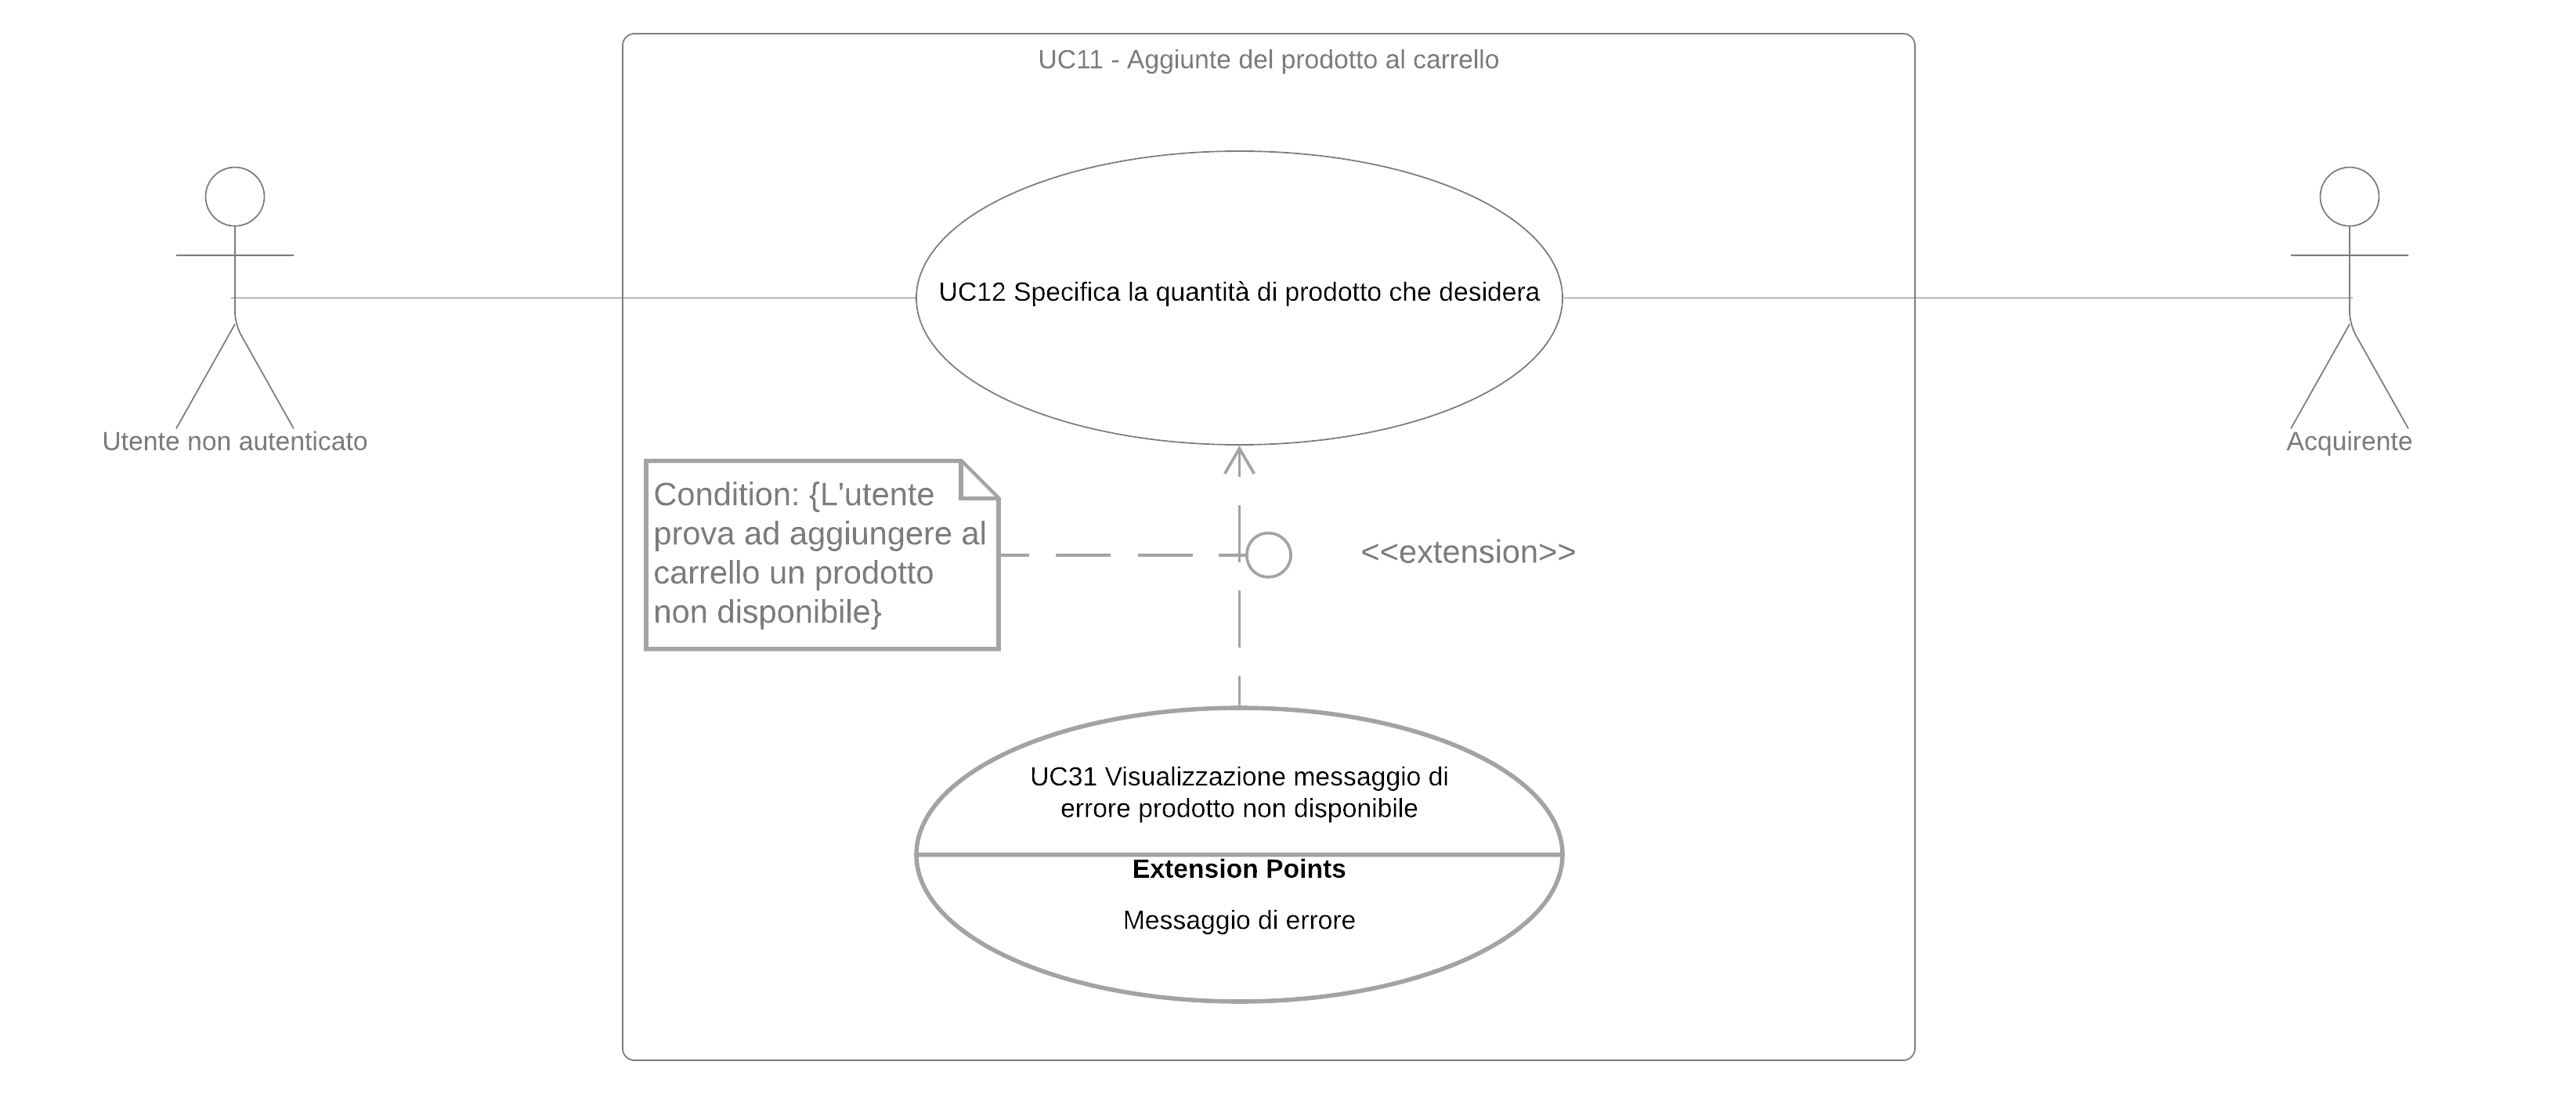
\includegraphics[width=\textwidth]{Immagini/DiagrammiUC/UC11AggiuntaProdottoAlCarrello.png}
    \caption{Diagramma di UC11: Aggiunta del prodotto al carrello} 
    \label{fig:Checkout}
\end{figure}


L'utente non autenticato o l'acquirente può aggiungere al carrello i prodotti.
\begin{itemize}
    \item \textbf{Attori Primari:} Acquirente; Utente non autenticato
    \item \textbf{Precondizione:} L'attore richiede di aggiungere una certa quantità del prodotto al carrello. 
    \item \textbf{Postcondizione:} L'attore ha aggiunto la quantità desiderata di prodotto al carrello.
    \item \textbf{Scenario Principale:} 
    \begin{itemize}
        \item (UC12) - Specifica la quantità di prodotto che desidera.
        \item L'attore aggiunge il prodotto al carrello.
        \item Il suo carrello personale viene aggiornato con il nuovo prodotto nella quantità indicata.
    \end{itemize}
    \item \textbf{Estensioni}:
    \begin{itemize}
        \item (UC31) - Visualizzazione messaggio di errore prodotto non disponibile.
    \end{itemize}
\end{itemize}

\subsection{UC12 - Modifica della quantità del prodotto}
\label{UC12}
L'acquirente o utente non autenticato modifica la quantità del prodotto che vuole nel carrello.
\begin{itemize}
    \item \textbf{Attori Primari:} Acquirente; Utente non autenticato.
    \item \textbf{Precondizione:} L'attore ha un prodotto che vuole nel carrello e desidera modificare la sua quantità.
    \item \textbf{Postcondizione:} La nuova quantità di prodotto da inserire nel carrello è aggiornata.
    \item \textbf{Scenario Principale:}
        \begin{itemize}
            \item L'attore chiede di modificare la quantità specificata di un certo prodotto.
            \item L'attore aumenta o diminuisce la quantità tra 1 e la disponibilità massima di prodotto.
            \item La nuova quantità di prodotto sarà quella fornita.
        \end{itemize}
    \item \textbf{Estensioni}:
    \begin{itemize}
        \item (UC32) - Visualizzazione messaggio di errore prodotto non disponibile.
    \end{itemize}
\end{itemize}

%% AGGIUNTA DI FILIPPO E LEONARDO ^

% 6. Checkout. The page where the user can:
%     a. Insert payment details;
%     b. Insert email address for the delivery of the notes;
%     c. Proceed to the payment;
% If the payment is successful the consumer will be redirected to the final step of the checkout
% process, where he can review the order just created. If the payment fails, the application will notify
% the consumer, and he can retry to insert again the payment details and retry the payment.
% In case of successful payment, the application will send the product(s) via email (previously inserted
% in the checkout process) to the customer;

\subsection{UC13 - \glo{Checkout}}
\label{UC13}

\begin{figure}[H]
    \centering
    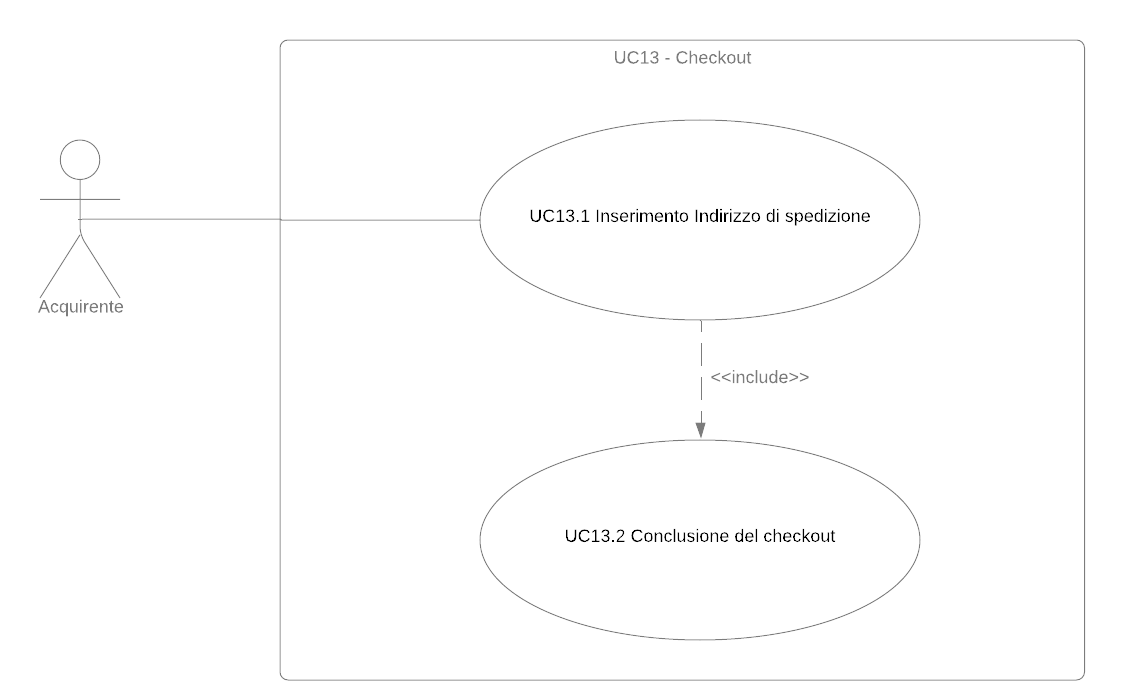
\includegraphics[scale=0.4]{Immagini/DiagrammiUC/UC13Checkout.png}
    \caption{Diagramma di UC13: Checkout} 
    \label{fig:Checkout}
\end{figure}

L'utente si trova nella pagina del carrello e vuole procedere al checkout per acquistare i prodotti scelti.
\begin{itemize}
    \item \textbf{Attori Primari:} Utente non autenticato; Acquirente e Stripe.
    \item \textbf{Precondizione:} L'acquirente o l'utente non autenticato si trova nella pagina del carrello.
    \item \textbf{Postcondizione:} L'utente ha terminato il checkout e si trova nella pagina di riepilogo ordine.
    \item \textbf{Scenario Principale:} L'attore si trova nella pagina del carrello e clicca sull'azione per iniziare il checkout. In seguito farà i seguenti passi:
    \begin{itemize}
        \item (UC13.1) - Inserimento indirizzo di spedizione.
        \item (UC13.2) - Conclusione checkout.
    \end{itemize}
    \item \textbf{Scenario Alternativo 1:} Se l'attore non è ancora autenticato, viene reindirizzato alla pagina del login (UC1.2) o della registrazione per autenticarsi come acquirente, per poi procede al checkout.
    \item \textbf{Scenario Alternativo 2:} Se l'utente non autenticato è stato reindirizzato alla pagina di login e accede come venditore, il carrello con i prodotti salvati viene svuotato.
    \item \textbf{Inclusioni:}
    \begin{itemize}
        \item (UC13.2) - Conclusione checkout.
    \end{itemize}
\end{itemize}
\newpage
\subsubsection{UC13.1 - Inserimento indirizzo di spedizione}
\label{UC13.1}
L'acquirente inserisce l'indirizzo al quale verrà spedito il pacco con l'ordine effettuato.
\begin{itemize}
    \item \textbf{Attori Primari:} Acquirente.
    \item \textbf{Precondizione:} Acquirente non ha ancora inserito l'indirizzo di spedizione.
    \item \textbf{Postcondizione:} Acquirente ha inserito l'indirizzo di spedizione e vengono calcolati e mostrati il costo della spedizione e i dazi doganali.
    \item \textbf{Scenario Principale:}
    \begin{itemize}
        \item (UC23.4) - L'acquirente inserisce l'indirizzo di spedizione obbligatorio.
        \item Vengono calcolati i costi di spedizione e i dazi doganali.
        \item Vengono mostrati i costi aggiuntivi appena calcolati.
        \item Dopo aver accettato anche i costi aggiuntivi, verrà reindirizzato alla pagina di Stripe.
    \end{itemize}
    \item \textbf{Estensioni:}
    \begin{itemize}
        \item (UC30) - Visualizzazione messaggio indirizzo di spedizione non inserito.
    \end{itemize}
\end{itemize}

\subsubsection{UC13.2 - Conclusione checkout}
\label{UC13.2}
L'acquirente procede al pagamento attraverso il servizio fornito da Stripe e poi gli viene mostrata una pagina con il resoconto dell'ordine.
\begin{itemize}
    \item \textbf{Attori Primari:} Acquirente e Stripe.
    \item \textbf{Precondizione:} L'acquirente non ha ancora pagato e il carrello non è vuoto.
    \item \textbf{Postcondizione:} L'acquirente ha effettuato il pagamento, il suo carrello è vuoto e si trova sulla pagina di riepilogo dell'ordine.
    \item \textbf{Scenario Principale:}
        \begin{itemize}
            \item L'acquirente viene indirizzato alla pagina di checkout di Stripe, dove pagherà il costo del carrello più le spese di spedizione e le tasse.
            \item Stripe si occupa del pagamento.
            \item Quando è avvenuto il pagamento viene svuotato il carrello e gli articoli che lo componevano vengono sottratti nella quantità acquistata da quelli disponibili e poi mostrati nella pagina di riepilogo ordine (UC14).
        \end{itemize}
    \item \textbf{Scenario Alternativo:} Se il pagamento fallisce l'utente viene riportato alla pagina del carrello, senza che questo venga svuotato.
\end{itemize}

\subsection{UC14 - Pagina di riepilogo ordine}
\label{UC14}
L'acquirente o il venditore vuole vedere i prodotti contenuti in un ordine, le loro quantità, l'indirizzo di spedizione e il prezzo totale di pagamento.
\begin{itemize}
    \item \textbf{Attori Primari:} Acquirente; Venditore.
    \item \textbf{Precondizione:} L'attore ha premuto sull'azione di visualizzazione del riepilogo di un ordine precedentemente fatto da un acquirente. 
    \item \textbf{Postcondizione:} Viene aperta la pagina di riepilogo ordine.
    \item \textbf{Scenario Principale:}
    \begin{itemize}
        \item L'attore preme sull'azione di visualizzazione del riepilogo.
        \item Vede i prodotti contenuti nell'ordine con le loro quantità, l'indirizzo di spedizione e il prezzo totale di pagamento.
    \end{itemize}
\end{itemize}
